\documentclass[border=3pt]{standalone}
% Preâmbulo compartilhado pelos diagramas TikZ da aula 5 de IHC (Processos de Design)
\usepackage[T1]{fontenc}
\usepackage[utf8]{inputenc}
\usepackage{lmodern}
\usepackage{amsmath}
\usepackage{xcolor}
\usepackage{tikz}
\usetikzlibrary{arrows.meta,angles,quotes,decorations.pathmorphing,calc,
                positioning,shapes.geometric,shapes.misc,backgrounds,fit,
                math}

% Paleta (mesma dos SVGs originais)
% Paleta da disciplina de IHC: acento roxo (#755099), da capa do livro.
% (o nome "dblue" é mantido para não alterar todos os diagramas)
\definecolor{dblue}{HTML}{755099}
\definecolor{dorange}{HTML}{B3541E}
\definecolor{dgreen}{HTML}{4A7C59}
\definecolor{dred}{HTML}{9C4B4B}
\definecolor{dcream}{HTML}{F4F1EA}
\definecolor{dshade}{HTML}{DDD7C9}

% Função gaussiana (não normalizada por padrão de escala visual)
\pgfmathdeclarefunction{gauss}{3}{%
  \pgfmathparse{1/(#3*sqrt(2*pi))*exp(-((#1-#2)^2)/(2*#3^2))}%
}

% Estilos comuns (prefixo d... para não colidir com chaves internas do pgf)
\tikzset{
  >={Stealth[length=2mm]},
  dguide/.style={gray!55, dashed, line width=0.4pt},
  daxis/.style={gray!60, line width=0.7pt, ->},
  dbody/.style={fill=black!3, draw=black!80, line width=1pt},
  dacc/.style={draw=dblue, line width=1pt},
  dlbl/.style={black!55, font=\small},
  dsub/.style={black!45, font=\footnotesize},
  dstate/.style={circle, draw=black!80, fill=dcream, line width=1pt,
                 minimum size=17mm, font=\large, inner sep=1pt},
  dobs/.style={circle, draw=black!80, fill=dshade, line width=1pt,
               minimum size=14mm, font=\large, inner sep=1pt},
  dbox/.style={rounded corners=2pt, draw=black!80, fill=dcream, line width=1pt,
               align=center, inner sep=6pt},
  dop/.style={circle, draw=black!80, fill=white, line width=1pt,
              minimum size=6mm, inner sep=0pt, font=\small},
  dtrans/.style={->, dblue, line width=1pt},
  dmeas/.style={->, dorange, line width=1pt},
  dcurve/.style={line width=1pt, dblue},
  dcurveb/.style={line width=1.4pt, dorange},
}

\begin{document}
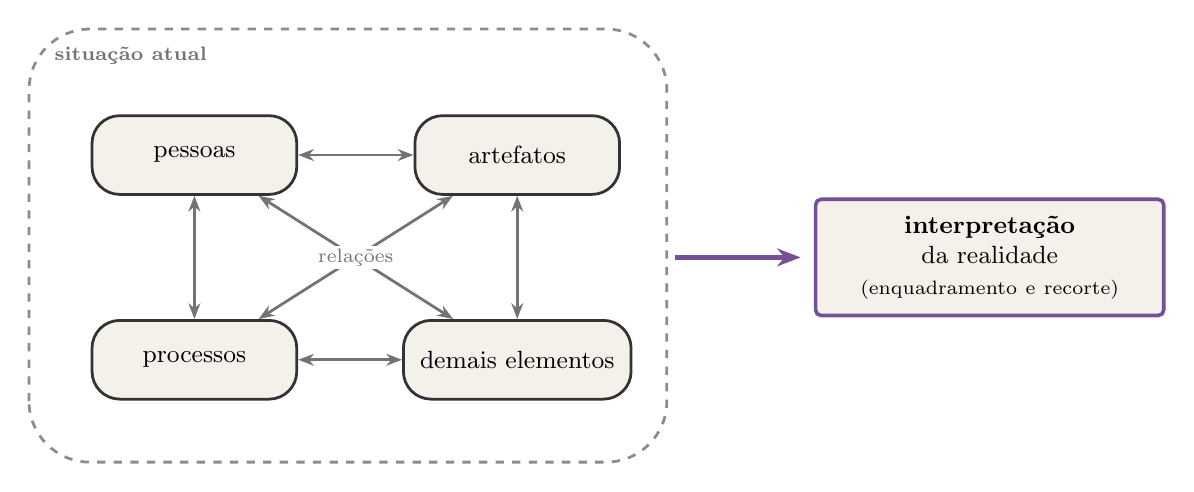
\begin{tikzpicture}[x=1cm,y=1cm,
   el/.style={dbox, rounded corners=10pt, minimum width=2.6cm, minimum height=1.0cm, font=\small}]

  \draw[black!45, dashed, rounded corners=22pt, line width=1pt] (-1.2,-2.6) rectangle (6.9,2.9);
  \node[dlbl, font=\scriptsize\bfseries, anchor=north west] at (-1.0,2.8) {situação atual};

  \node[el] (p) at (0.9,1.3) {pessoas};
  \node[el] (a) at (5.0,1.3) {artefatos};
  \node[el] (pr) at (0.9,-1.3) {processos};
  \node[el] (r) at (5.0,-1.3) {demais elementos};
  \draw[<->, black!55, line width=1pt] (p) -- (a); \draw[<->, black!55, line width=1pt] (p) -- (pr);
  \draw[<->, black!55, line width=1pt] (a) -- (r); \draw[<->, black!55, line width=1pt] (pr) -- (r); \draw[<->, black!55, line width=1pt] (p) -- (r); \draw[<->, black!55, line width=1pt] (a) -- (pr);
  \node[dlbl, font=\scriptsize, fill=white, inner sep=1pt] at (2.95,0) {relações};

  % lente / foco
  \draw[dtrans, line width=1.6pt, -{Stealth[length=3mm]}] (7.0,0) -- (8.6,0);
  \node[dbox, draw=dblue, line width=1.3pt, text width=4.0cm, font=\small, align=center] (i) at (11.0,0) {\textbf{interpretação}\\ da realidade\\ \scriptsize (enquadramento e recorte)};


\end{tikzpicture}
\end{document}
